%%%%%%%%%%%%%%%%%%%%%%%%%%%%%%%%%%%%%%%%
%% HOWTO                              %%
%%                                    %%
%% start the tree with \section       %%
%% do not use \chapter                %%
%% use \newpage between each \section %%
%%                                    %%
\if{0}
%% to insert pictures, use            %%
    \vspace{1cm} \begin{figure}[!h] \centering \includegraphics{.png} \caption{} \end{figure}
%%                                    %%
\fi
%%%%%%%%%%%%%%%%%%%%%%%%%%%%%%%%%%%%%%%%


\newcommand{\culdelampe}[0]{
        \begin{figure}[!h] \centering 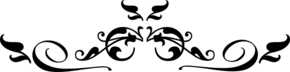
\includegraphics[height=1cm]{swirl.png} \end{figure}
}


\section{Introduction}

{\fontfamily{pzc}\selectfont \textit{Il faisait nuit, et moi du vélo.}}\\
\hbox{}\hfill {\small Joseph Marchand}

Antoine arrivait à quatre heures, à pied et à marcher, du bowling où il avait explosé le score de ses adversaires ainsi que la plupart des quilles.

QUAND SOUDAIN.

Une soucoupe volante lui traversa l'esprit puis le pied droit. Il dut alors recourir aux mains et au commissariat. Il s'arrêta alors : on le prendrait pour fou et pour exemple. Il prit alors son courage à deux mains et son laptop dans la troisième, et se mit à chercher sur Internet des forums racontant des expériences similaires, afin de pouvoir réagir en conséquence.

De cet étrange astronef s'échappa une lueur éclatant le paysage et les vitres alentour. Il entendit une voix qui lui tint à peu près ce langage, parlant en anglais mais surtout en gesticulant : \og TOUDOU \fg. Ignorant cette langue et même la bouche se trouvant autour, il se concentra plutôt sur le vaisseau : celui-ci lui parut constituer un \textbf{feu d'artifice} de failles autant de sécurité que spatio-temporelles.

Tel un pirate sorti d'un film de Michael Bay, quelques minutes accompagnées de Jammie Dodgers lui suffirent pour se balader dans l'engin puis dans l'espace. Il décida alors : et si je conquérais la Lune ? Mais pourquoi s'arrêter là ? De plus, je pourrais construire d'autres vaisseaux sur d'autres planètes que je coloniserais ? Et peut-être que tout cela me donnerait une idée de sujet de concours\footnote{\url{http://aichallenge.org}} ?

Connaissant la position précise des planètes se trouvant dans le système solaire ambiant, vous cherchez à répartir vos constructions de vaisseaux stratégiquement afin de vous assurer l'hégémonie hyperspatiale et autres mots compliqués.

\newpage

\section{Votre mission}

{\fontfamily{pzc}\selectfont \textit{L'ennemi est bête. Il croit que c'est nous l'ennemi, alors que c'est lui ! J'en ris encore !}}\\
\hbox{}\hfill {\small Pierre Desproges}

Vous conduisez un ensemble de vaisseaux spatiaux qui vous permettent de tuer les vaisseaux ennemis, ainsi que les trente-six prochaines heures. Ces vaisseaux permettent également de construire des phrases redondantes ou de coloniser d'autres planètes, qui à leur tour produiront des vaisseaux. En somme, un sacré bazar.

Une planète plus grosse produisant plus de vaisseaux par tour, vous devez bien choisir les différentes planètes à coloniser. De plus, le temps d'accès d'une planète à une autre est proportionnel à la distance qui les sépare ainsi qu'à votre capacité à coder sans bugs\footnote{Plutôt limitée, à ce que nous avons pu voir pendant les épreuves régionales.}.

N'oubliez pas que pendant que vous colonisez gaiement, un autre candidat dans la salle\footnote{Lui, là, à droite.} essaie de se tailler la part du lion et du gâteau. Si vous cherchez à attaquer une planète avec $n$ vaisseaux ennemis alors que vous en avez $m \leqslant n$, vous perdrez la bataille\footnote{Et pas que.} et il lui en restera $n - m$. Si vous avez $m > n$ vaisseaux, vous remporterez le match et la planète en prime, et il vous restera $m - n$ vaisseaux.

Le gagnant est celui qui à l'issue des 500 tours a le plus de vaisseaux. En cas d'égalité, les deux joueurs disputeront une partie de TetriNET pour déterminer le vainqueur.